\documentclass[tikz,border=3pt]{standalone}
\usepackage[utf8]{inputenc}
\usepackage[T1]{fontenc}
\usepackage{lmodern}
\renewcommand{\familydefault}{\sfdefault}
\usepackage{sansmath}\sansmath
\usepackage{chemfig}
\usepackage{pgfplots}\pgfplotsset{compat=1.18,/pgf/number format/use comma,/pgf/number format/1000 sep={.}}
\usetikzlibrary{arrows.meta,calc,positioning,decorations.pathmorphing,patterns}
% paleta del sitio
\definecolor{nar}{HTML}{E8680C}\definecolor{narc}{HTML}{FFB35C}\definecolor{hielo}{HTML}{FFF3E8}
\definecolor{tinta}{HTML}{1D1D1F}\definecolor{gris}{HTML}{6E6E73}\definecolor{lila}{HTML}{7C5CF0}
\definecolor{azul}{HTML}{2F6FD6}\definecolor{menta}{HTML}{17A673}\definecolor{coral}{HTML}{E8342A}
% vaso de precipitados centrado en x, base en y
\newcommand{\vaso}[2]{%
  \fill[azul!12] (#1-0.9,#2) rectangle (#1+0.9,#2+1.3);
  \draw[tinta,thick] (#1-1.0,#2+1.85) -- (#1-0.9,#2+1.75) -- (#1-0.9,#2) -- (#1+0.9,#2) -- (#1+0.9,#2+1.85);
  \draw[azul!60] (#1-0.9,#2+1.3) -- (#1+0.9,#2+1.3);}
\begin{document}
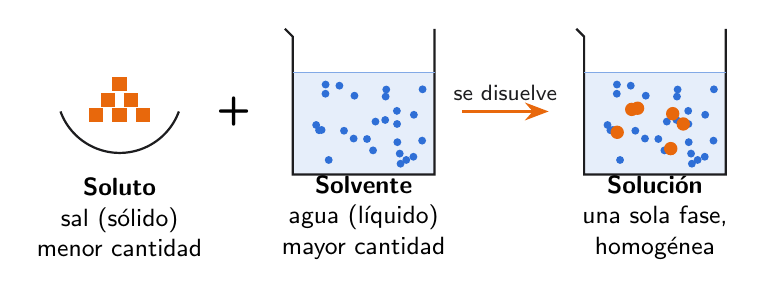
\begin{tikzpicture}[font=\small]
% soluto: cristales en un vidrio de reloj
\begin{scope}[shift={(0,0.45)}]
\draw[tinta,thick] (-0.75,0.35) arc[start angle=200,end angle=340,radius=0.8];
\foreach \x/\y in {-0.3/0.3,0/0.3,0.3/0.3,-0.15/0.5,0.15/0.5,0/0.7}
  \fill[nar] (\x-0.09,\y-0.09) rectangle (\x+0.09,\y+0.09);
\end{scope}
\node[align=center] at (0,-0.55) {\textbf{Soluto}\\sal (sólido)\\menor cantidad};
\node[font=\Large\bfseries] at (1.45,0.8) {+};
% solvente
\vaso{3.1}{0}
\pgfmathsetseed{4}
\foreach \i in {1,...,26} {\fill[azul] ($(3.1,0)+(-0.8+1.6*rnd,0.1+1.1*rnd)$) circle (0.05);}
\node[align=center] at (3.1,-0.55) {\textbf{Solvente}\\agua (líquido)\\mayor cantidad};
\draw[-{Stealth[length=3mm]},very thick,nar] (4.35,0.8) -- (5.45,0.8) node[midway,above,tinta,font=\footnotesize] {se disuelve};
% solucion
\vaso{6.8}{0}
\pgfmathsetseed{4}
\foreach \i in {1,...,26} {\fill[azul] ($(6.8,0)+(-0.8+1.6*rnd,0.1+1.1*rnd)$) circle (0.05);}
\pgfmathsetseed{11}
\foreach \i in {1,...,6} {\fill[nar] ($(6.8,0)+(-0.75+1.5*rnd,0.15+1.0*rnd)$) circle (0.085);}
\node[align=center] at (6.8,-0.55) {\textbf{Solución}\\una sola fase,\\homogénea};
\end{tikzpicture}
\end{document}
